\documentclass[11pt,letterpaper]{article}
\usepackage{ifthen}
\usepackage{amssymb}
\usepackage{graphicx}
\usepackage{tikz}
\usepackage{algorithm}
\usepackage{algpseudocode}
\usepackage[numbers,sort&compress]{natbib}
% Shared house style for the AI Trading 24/7 modular documents.
% Every module \input's this file, then sets its own \title block and body.
% Derived from the former InfrastructureSetup.tex / ReplicationExecutionFlow.tex preambles.

% Beamer supplies its own page layout, headings, lists, and page furniture.
\newif\ifaitradingbeamer
\makeatletter
\@ifclassloaded{beamer}{\aitradingbeamertrue}{\aitradingbeamerfalse}
\makeatother
\ifaitradingbeamer\else
\usepackage[top=1in, bottom=1in, left=1.1in, right=1.1in]{geometry}
\fi
\usepackage{microtype}
\usepackage{libertine}
\usepackage[libertine]{newtxmath}
\usepackage[T1]{fontenc}
\usepackage{amsmath}
\ifaitradingbeamer\else
\usepackage{enumitem}
\usepackage{setspace}
\usepackage{titlesec}
\fi
\usepackage{xcolor}
\ifaitradingbeamer\else
\usepackage{fancyhdr}
\fi
\usepackage{longtable}
\usepackage{booktabs}
\usepackage{array}
\usepackage{tabularx}
\usepackage{seqsplit}
\usepackage{hyperref}
\usepackage{xurl}

% Colors
\definecolor{uablue}{RGB}{0,56,107}
\definecolor{sectiongray}{RGB}{64,64,64}
\definecolor{accent}{RGB}{150,0,24}
\definecolor{definitiongreen}{RGB}{0,102,51}

% Header (each module may override \fancyhead[L] after \input if it wishes)
\ifaitradingbeamer\else
\pagestyle{fancy}
\fancyhf{}
\fancyhead[L]{\small\textcolor{uablue}{AI Trading 24/7: Step-by-Step Build}}
\fancyhead[R]{\small\textcolor{uablue}{Muting (Don) Ma}}
\fancyfoot[C]{\thepage}
\renewcommand{\headrulewidth}{0.5pt}

% Section format
\titleformat{\section}
  {\color{uablue}\normalfont\large\bfseries}
  {\thesection.}{0.5em}{}[\color{uablue}\titlerule]
\titleformat{\subsection}
  {\color{sectiongray}\normalfont\normalsize\bfseries}
  {\thesubsection}{0.5em}{}
\titlespacing*{\section}{0pt}{1.4ex plus 0.5ex minus .2ex}{0.8ex plus .2ex}
\titlespacing*{\subsection}{0pt}{1.0ex plus 0.4ex minus .2ex}{0.5ex plus .2ex}
\newcommand{\sectionbreak}{\clearpage}

\setstretch{1.08}
\setlength{\parskip}{0.45em}
\setlength{\parindent}{0pt}
\fi
\setlength{\emergencystretch}{3em}
\hypersetup{colorlinks=true, linkcolor=uablue, urlcolor=uablue,
  citecolor=accent, filecolor=accent, menucolor=uablue,
  linktoc=all, breaklinks=true}

% Shared macros (superset of those used by the two former documents)
\newcolumntype{L}{>{\raggedright\arraybackslash}X}
\newcolumntype{C}{>{\centering\arraybackslash}X}
\newcommand{\hd}[1]{\textbf{\textcolor{uablue}{#1}}}
\newcommand{\callout}[1]{\begin{center}\fcolorbox{uablue}{white}{\parbox{0.96\linewidth}{\small #1}}\end{center}}
\newcommand{\code}[1]{\texttt{\seqsplit{#1}}}
\newcommand{\yes}{\textcolor{definitiongreen}{\textbf{Yes}}}
\newcommand{\no}{\textcolor{accent}{\textbf{No}}}
\newcommand{\have}{\textcolor{definitiongreen}{\textbf{HAVE}}}
\newcommand{\wip}{\textcolor{accent}{\textbf{PARTIAL}}}
\newcommand{\build}{\textcolor{accent}{\textbf{BUILD}}}
\newcommand{\blank}{\textcolor{accent}{\framebox[0.8em]{\rule{0pt}{0.66em}}}}

% Title block helper: \aitradingtitle{TITLE}{SUBTITLE}{DRAFT LINE}
\newcommand{\aitradingtitle}[3]{%
  \begin{center}
    \Large\bfseries\color{uablue}#1\\[0.2em]
    \normalsize\color{black}#2\\[0.3em]
    \small Muting (Don) Ma, Ph.D.\\
    \small #3
  \end{center}
  \vspace{-0.2em}
}

% No page break before each section.
\renewcommand{\sectionbreak}{}
\newboolean{draftmode}
\setboolean{draftmode}{false}
% ============================================================================
% AUTOMATIC COUNTER CONTROL FOR SECTION MANAGEMENT
% ============================================================================
%
% This file automatically increments summary counters when you use
% standard LaTeX section commands. No manual intervention needed!
%
% The counters will automatically update when you use:
% \section{...}, \subsection{...}, \subsubsection{...}
% ============================================================================

% Hook into section counter increments instead of redefining commands
\makeatletter

% Define counters first (if not already defined)
\@ifundefined{c@SumSection}{\newcounter{SumSection}}{}
\@ifundefined{c@SumSubsection}{\newcounter{SumSubsection}[SumSection]}{}
\@ifundefined{c@SumSubsubsection}{\newcounter{SumSubsubsection}[SumSubsection]}{}
\@ifundefined{c@SumPara}{\newcounter{SumPara}[SumSubsubsection]}{}
\@ifundefined{c@SumFin}{\newcounter{SumFin}[SumSubsubsection]}{}
\@ifundefined{c@SumTodo}{\newcounter{SumTodo}[SumSubsubsection]}{}

% Create a flag to detect bibliography
\newif\if@inbibliography
\@inbibliographyfalse

% Hook into the bibliography environment
\let\old@bibliography\bibliography
\renewcommand{\bibliography}[1]{%
  \@inbibliographytrue
  \old@bibliography{#1}%
  \@inbibliographyfalse
}

% Only redefine thebibliography if it exists (not all document classes have it)
\@ifundefined{thebibliography}{}{%
  \let\old@thebibliography\thebibliography
  \renewcommand{\thebibliography}[1]{%
    \@inbibliographytrue
    \old@thebibliography{#1}%
  }
}

\@ifundefined{endthebibliography}{}{%
  \let\old@endthebibliography\endthebibliography
  \renewcommand{\endthebibliography}{%
    \old@endthebibliography
    \@inbibliographyfalse
  }
}

% Hook into the section counter increments
\let\old@stepcounter\stepcounter
\renewcommand{\stepcounter}[1]{%
  \old@stepcounter{#1}%
  % Only track if not in bibliography
  \if@inbibliography\else
    \def\@tmpa{#1}%
    \def\@tmpb{section}%
    \ifx\@tmpa\@tmpb
      \stepcounter{SumSection}%
      \setcounter{SumSubsection}{0}%
      \setcounter{SumSubsubsection}{0}%
      \setcounter{SumPara}{0}%
      \setcounter{SumFin}{0}%
      \setcounter{SumTodo}{0}%
    \fi
    \def\@tmpb{subsection}%
    \ifx\@tmpa\@tmpb
      \stepcounter{SumSubsection}%
      \setcounter{SumSubsubsection}{0}%
      \setcounter{SumPara}{0}%
      \setcounter{SumFin}{0}%
      \setcounter{SumTodo}{0}%
    \fi
    \def\@tmpb{subsubsection}%
    \ifx\@tmpa\@tmpb
      \stepcounter{SumSubsubsection}%
      \setcounter{SumPara}{0}%
      \setcounter{SumFin}{0}%
      \setcounter{SumTodo}{0}%
    \fi
  \fi
}

\makeatother

% Quick reset command for beginning of document
\newcommand\resetallcounters{%
  \setcounter{SumSection}{0}%
  \setcounter{SumSubsection}{0}%
  \setcounter{SumSubsubsection}{0}%
  \setcounter{SumPara}{0}%
  \setcounter{SumFin}{0}%
  \setcounter{SumTodo}{0}%
}

% Initialize counters at document start
\resetallcounters

% Utility command to display current counter values (for debugging)
\newcommand\showcounters{%
  \ifthenelse{\boolean{draftmode}}{%
    \marginpar{\tiny Counter: \arabic{SumSection}-\arabic{SumSubsection}-\arabic{SumSubsubsection}-\arabic{SumPara}}%
  }{}%
}

% Help command for quick reference
\newcommand\sumhelp{%
  \typeout{========================================}%
  \typeout{SUMMARY CONTROL USAGE EXAMPLES:}%
  \typeout{Counters auto-increment with sections!}%
  \typeout{1. Marker-based: \string\sump\space Text here \string\sumpe}%
  \typeout{2. Brace-based: \string\sumparab{Text here}}%
  \typeout{3. TODO marker: \string\todostart\space Task \string\todoend}%
  \typeout{========================================}%
}

% ============================================================================
% USAGE DOCUMENTATION FOR SUMCONTROL COMMANDS
% ============================================================================
%
% MARKER-BASED COMMANDS (no braces needed):
% ------------------------------------------
% 1. Summary paragraphs:
%    \sump This is my summary text. \sumpe  (short version)
%    \sumpara This is my summary text. \sumparaend (long version)
%
% 2. TODO markers:
%    \todostart This needs to be done. \todoend
%
% BRACE-BASED COMMANDS (alternative syntax):
% -------------------------------------------
% 1. Summary paragraphs with braces:
%    \sumparab{This is my summary text}
%
% 2. TODO items with braces:
%    \todob{This needs to be done}
%
% 3. Final paragraphs (always shown):
%    \finalpara{This text is always displayed}
%
% AUTOMATIC COUNTER MANAGEMENT:
% -----------------------------
% Counters automatically increment when you use \section, \subsection, etc.
% No manual counter commands needed!
%
% DRAFT/FINAL MODE:
% -----------------
% Set \setboolean{draftmode}{true} for draft (shows markers)
% Set \setboolean{draftmode}{false} for final (hides markers)
% ============================================================================

% Counter definitions removed - now in SumCounterControl.tex
% The counters are defined in SumCounterControl.tex which must be loaded

% Helper macros for final mode (defined outside ifthenelse to avoid parameter nesting issues)
\long\def\SumControlGobbleSumPara#1\sumparaend{}
\long\def\SumControlGobbleSump#1\sumpe{}
\newcommand\SumControlTodoBFinal[1]{%
  \PackageWarning{main}{TODO item still present: #1}%
  \stepcounter{SumTodo}%
  \fcolorbox{gray}{red}{\bfseries\sffamily\scriptsize TODO\arabic{SumSection}-\arabic{SumSubsection}-\arabic{SumSubsubsection}-\arabic{SumTodo}}%
  $\blacktriangleright$#1%
}

% Marker-based sumpara commands (no braces needed)
% Usage: \sumpara This is my sentence. \sumparaend
% Or simply: \sp This is my sentence. \spe
\ifthenelse{\boolean{draftmode}}{
  % Draft mode: show colored markers
  \newcommand\sumpara{%
    \stepcounter{SumPara}%
    \fcolorbox{gray}{green}{\bfseries\sffamily\scriptsize Sum\arabic{SumSection}-\arabic{SumSubsection}-\arabic{SumSubsubsection}-\arabic{SumPara}}%
    $\blacktriangleright$\color{red}\slshape%
  }
  \newcommand\sumparaend{\normalfont\color{black}$\blacktriangleleft$}
  % Short aliases (avoid \sp which is already defined in LaTeX)
  \newcommand\sump{\sumpara}
  \newcommand\sumpe{\sumparaend}
}{
  % Final mode: hide content between markers (gobble content)
  \let\sumpara\SumControlGobbleSumPara
  \newcommand\sumparaend{}
  \let\sump\SumControlGobbleSump
  \newcommand\sumpe{}
}

% TODO markers (same pattern)
\ifthenelse{\boolean{draftmode}}{
  \newcommand\todostart{%
    \stepcounter{SumTodo}%
    \fcolorbox{gray}{red}{\bfseries\sffamily\scriptsize TODO\arabic{SumSection}-\arabic{SumSubsection}-\arabic{SumSubsubsection}-\arabic{SumTodo}}%
    $\blacktriangleright$\color{blue}\slshape%
  }
  \newcommand\todoend{\normalfont\color{black}$\blacktriangleleft$}
}{
  \newcommand\todostart{%
    \PackageWarning{main}{TODO marker still present}%
    \stepcounter{SumTodo}%
    \fcolorbox{gray}{red}{\bfseries\sffamily\scriptsize TODO\arabic{SumSection}-\arabic{SumSubsection}-\arabic{SumSubsubsection}-\arabic{SumTodo}}%
    $\blacktriangleright$%
  }
  \newcommand\todoend{}
}

% Final/Fixed sentence markers (cyan box, black text)
% Usage: \finpara This is my fixed sentence. \finparaend
% Or simply: \fin This is my sentence. \fine
\ifthenelse{\boolean{draftmode}}{
  % Draft mode: show cyan markers with black text
  \newcommand\finpara{%
    \stepcounter{SumFin}%
    \fcolorbox{gray}{cyan}{\bfseries\sffamily\scriptsize Fin\arabic{SumSection}-\arabic{SumSubsection}-\arabic{SumSubsubsection}-\arabic{SumFin}}%
    $\blacktriangleright$%
  }
  \newcommand\finparaend{$\blacktriangleleft$}
  % Short aliases
  \newcommand\fin{\finpara}
  \newcommand\fine{\finparaend}
}{
  % Final mode: empty commands, content shows through
  \newcommand\finpara{}
  \newcommand\finparaend{}
  \newcommand\fin{}
  \newcommand\fine{}
}

% Keep the brace-based versions as alternatives (backward compatibility)
\ifthenelse{\boolean{draftmode}}{
  \newcommand\sumparab[1]{%
    \stepcounter{SumPara}%
    \fcolorbox{gray}{green}{\bfseries\sffamily\scriptsize Sum\arabic{SumSection}-\arabic{SumSubsection}-\arabic{SumSubsubsection}-\arabic{SumPara}}%
    {$\blacktriangleright$\textcolor{red}{\textsl{#1}}$\blacktriangleleft$}%
  }
  \newcommand\todob[1]{%
    \stepcounter{SumTodo}%
    \fcolorbox{gray}{red}{\bfseries\sffamily\scriptsize TODO\arabic{SumSection}-\arabic{SumSubsection}-\arabic{SumSubsubsection}-\arabic{SumTodo}}%
    {$\blacktriangleright$\textcolor{blue}{\textsl{#1}}$\blacktriangleleft$}%
  }
  \newcommand\finparab[1]{%
    \stepcounter{SumFin}%
    \fcolorbox{gray}{cyan}{\bfseries\sffamily\scriptsize Fin\arabic{SumSection}-\arabic{SumSubsection}-\arabic{SumSubsubsection}-\arabic{SumFin}}%
    {$\blacktriangleright$#1$\blacktriangleleft$}%
  }
}{
  \newcommand\sumparab[1]{}
  \let\todob\SumControlTodoBFinal
  \newcommand\finparab[1]{#1}
}

% finalpara stays the same - just outputs content
\newcommand\finalpara[1]{#1}

% ============================================================================
% AUTHOR NOTES AND COMMENTS SYSTEM
% ============================================================================
%
% USAGE:
% ------
% Each author can have their own comment command:
% \dm{This is DM's comment}
% \mh{This is MH's comment}
% \my{This is MY's comment}
%
% Add more authors as needed following the same pattern.
%
% DRAFT/FINAL MODE:
% -----------------
% Comments are shown/hidden based on the draftmode boolean from SumControl.tex
% ============================================================================


% DM (Don Ma) comments
\newcounter{DMComments}
\setcounter{DMComments}{0}
\ifthenelse{\boolean{draftmode}}{
  \newcommand\dm[1]{%
    \stepcounter{DMComments}%
    \fcolorbox{gray}{yellow}{\bfseries\sffamily\scriptsize DM\arabic{DMComments}}%
    {$\blacktriangleright$\textcolor{green!60!black}{\textsl{#1}}$\blacktriangleleft$}%
  }
}{
  \newcommand\dm[1]{%
    \stepcounter{DMComments}%
    \fcolorbox{gray}{yellow}{\bfseries\sffamily\scriptsize DM\arabic{DMComments}}%
    {$\blacktriangleright$\textcolor{green!60!black}{\textsl{#1}}$\blacktriangleleft$}%
  }
}

% Generic author comment template
% Copy and modify for additional authors:
% \newcounter{XXComments}
% \setcounter{XXComments}{0}
% \ifthenelse{\boolean{draftmode}}{
%   \newcommand\xx[1]{\stepcounter{XXComments}\nb{XX\arabic{XXComments}}{\textcolor{purple}{\textsl{#1}}}}
% }{
%   \newcommand\xx[1]{}
% }

\usepackage{cleveref}
\hypersetup{pdftitle={A Fixed Iterated Greedy Sequence Keeps Its Mean Weighted-Tardiness Advantage under Processing-Time Variability in a Flow Shop with Release Dates},
  pdfauthor={Muting (Don) Ma},colorlinks=true,linkcolor=uablue,urlcolor=uablue,
  citecolor=accent,filecolor=accent,menucolor=uablue,linktoc=all,breaklinks=true}
\fancyhead[L]{\small\textcolor{uablue}{Fixed iterated greedy sequences under processing-time variability}}
\setlength{\headheight}{14pt}
\graphicspath{{../results/}}
\renewcommand{\arraystretch}{1.15}
\numberwithin{equation}{section}
\crefname{algorithm}{Algorithm}{Algorithms}

% Job weight shading for the Gantt charts: one blue hue, light to dark as weight grows.
\definecolor{ink}{HTML}{19354A}
\definecolor{muted}{HTML}{536878}
\definecolor{gridgray}{HTML}{E4E3DF}
\definecolor{w1}{HTML}{9EC5F4}
\definecolor{w2}{HTML}{3987E5}
\definecolor{w4}{HTML}{184F95}
\colorlet{lab1}{ink}
\colorlet{lab2}{ink}
\colorlet{lab4}{white}
% \gantt{list of job/stage/start/completion/weight}: one schedule on four stages, 0 to 140 minutes.
\newcommand{\gantt}[1]{%
\begin{tikzpicture}[x=0.095cm,y=0.38cm]
  \foreach \t in {0,20,...,140} {
    \draw[gridgray,line width=0.4pt] (\t,0) -- (\t,-4);
    \node[font=\scriptsize,text=muted,anchor=north] at (\t,-4) {\t};}
  \foreach \s in {1,...,4}
    \node[font=\footnotesize,text=muted,anchor=east] at (-1,-\s+0.5) {S\s};
  \foreach \j/\s/\a/\b/\w in #1 {
    \fill[w\w] (\a+0.3,-\s+0.1) rectangle (\b-0.3,-\s+0.9);
    \node[font=\scriptsize\bfseries,text=lab\w] at ({(\a+\b)/2},-\s+0.5) {\j};}
\end{tikzpicture}}
\newcommand{\eddschedule}{1/1/13/24/2, 1/2/24/34/2, 1/3/34/40/2, 1/4/40/52/2,
  2/1/24/38/1, 2/2/38/47/1, 2/3/47/60/1, 2/4/60/73/1,
  5/1/45/62/1, 5/2/62/65/1, 5/3/65/70/1, 5/4/73/82/1,
  3/1/62/72/4, 3/2/72/75/4, 3/3/75/94/4, 3/4/94/108/4,
  6/1/78/83/2, 6/2/83/98/2, 6/3/98/101/2, 6/4/108/116/2,
  4/1/83/95/4, 4/2/98/111/4, 4/3/111/128/4, 4/4/128/139/4}
\newcommand{\igschedule}{1/1/13/24/2, 1/2/24/34/2, 1/3/34/40/2, 1/4/40/52/2,
  2/1/24/38/1, 2/2/38/47/1, 2/3/47/60/1, 2/4/60/73/1,
  3/1/51/61/4, 3/2/61/64/4, 3/3/64/83/4, 3/4/83/97/4,
  4/1/66/78/4, 4/2/78/91/4, 4/3/91/108/4, 4/4/108/119/4,
  6/1/78/83/2, 6/2/91/106/2, 6/3/108/111/2, 6/4/119/127/2,
  5/1/83/100/1, 5/2/106/109/1, 5/3/111/116/1, 5/4/127/136/1}

\begin{document}
\begin{center}
{\LARGE\bfseries\color{uablue} A Fixed Iterated Greedy Sequence Keeps Its Mean Weighted-Tardiness Advantage under Processing-Time Variability in a Flow Shop with Release Dates\par}
\vspace{0.8em}
{\large Muting (Don) Ma\par}
\vspace{0.2em}
{\small The University of Alabama, Tuscaloosa, AL, USA\par}
{\small \href{mailto:mma10@ua.edu}{mma10@ua.edu}\par}
\end{center}

\begin{abstract}
\noindent
\sumpara A planner who must fix one job order needs to know whether a searched order keeps its advantage over a dispatching rule once processing times vary. \sumparaend
\fin A planner who sequences jobs on a flow line where jobs cannot pass one another must commit to one job order before the processing times are known. \fine
\fin I compare the earliest due date (EDD) rule, a dispatching rule widely used in practice, with the iterated greedy algorithm of Ruiz and St\"utzle adapted to an eight-stage permutation flow shop with release dates and total weighted tardiness. \fine
\fin On instances with 15, 45, and 120~jobs, iterated greedy reduces total weighted tardiness relative to EDD by 98.5, 97.6, and 81.0~percent, and a mixed-integer program solved with HiGHS proves its values optimal on the instances with 6 and 15~jobs. \fine
\fin I then execute both fixed sequences on 180 paired scenarios of the 45-job instance in which each processing time is multiplied by an independent lognormal factor with mean one. \fine
\fin At a coefficient of variation of 0.2, the iterated greedy sequence has the lower weighted tardiness in all 30~scenarios, with a mean of 420.6 weighted minutes against 3,541.1, an 88.1~percent reduction. \fine
\fin As the coefficient of variation rises from 0.1 to 0.8, the relative reduction falls from 94.6 to 27.2~percent while the mean absolute reduction stays between 2,572.0 and 3,683.7 weighted minutes; at 0.8, the 10th percentile of the paired reduction falls to 851.5 weighted minutes and EDD is better in 1 of 30~scenarios. \fine
\fin Processing-time variability therefore erodes the advantage of the searched sequence first in the worst periods, while its mean advantage persists across the range tested. \fine
\end{abstract}

\noindent\textbf{Keywords:} Scheduling; Permutation flow shop; Weighted tardiness; Iterated greedy; Stochastic processing times

\section{Introduction}\label{sec:introduction}

\sumpara A planner on a flow line must commit to one job order before processing times are known, and the common dispatching rule ignores most of the information the planner holds. \sumparaend
\fin On flow lines such as printed circuit board assembly or furniture finishing, every job visits the same stages in the same order, and when jobs cannot pass one another, the order chosen at the first stage holds at every stage. \fine
\fin A job that is quick at the first stage and slow at a later one then delays every job behind it, and the resulting waiting accumulates downstream. \fine
\fin The planner of such a line fixes one sequence for the jobs of a planning period before processing begins, although the jobs are released at different times, carry due dates of unequal importance, and take processing times that will differ from their planned values. \fine
\fin Dispatching rules are used very often in practice, and the earliest due date (EDD) rule is among the most common rules for tardiness objectives~\cite{vallada2008review}. \fine
\fin EDD orders the jobs by due date alone, so it cannot account for job weights, release dates, or processing times at the stages after the first. \fine

\sumpara Searched sequences are known to beat dispatching rules on exact data, but whether that advantage survives variable processing times has been studied only for the makespan. \sumparaend
\fin Minimizing total tardiness in a permutation flow shop is NP-hard in the ordinary sense with one machine and in the strong sense with two or more~\cite{vallada2008review}, and the iterated greedy algorithm of \citet{ruiz2008igwt} was the best of the methods its authors tested for weighted tardiness. \fine
\fin That evaluation, like the review of \citet{vallada2008review}, used instances with fixed processing times and no release dates. \fine
\fin Studies of flow shops with random processing times have concentrated on the expected makespan, for which heuristics adapted from deterministic procedures, including sequences computed from mean processing times, perform close to the best stochastic methods~\cite{baker2012stochastic,framinan2015stochastic,juan2014simheuristic}, and a review of 100 studies of flow shops under uncertainty identifies tardiness and its weighted form as criteria that remain to be examined~\cite{gonzalezneira2017review}. \fine
\fin A broader review of schedule execution concludes that optimized predictive schedules outperform simple rules when uncertainty is low and lose that advantage beyond a level of variability that depends on the system~\cite{aytug2005executing}. \fine
\fin For weighted tardiness with release dates, it therefore remains open whether a searched sequence, held fixed, keeps its advantage over the EDD sequence as processing times vary, and at which level of variability that advantage weakens. \fine

\sumpara We compare the two fixed sequences on exact data, certify small optima, and execute both on paired scenarios across a range of variability. \sumparaend
\fin We adapt the iterated greedy algorithm of \citet{ruiz2008igwt} to an eight-stage permutation flow shop with release dates and total weighted tardiness, and we compare it with EDD on four synthetic instances with 6 to 120~jobs. \fine
\fin A mixed-integer program solved with HiGHS~\cite{highs} certifies the optimal values of the two smallest instances, and a checker that shares no code with either method recomputes the feasibility and the measures of every schedule. \fine
\fin We then execute both sequences, unchanged, on 180 paired scenarios of the 45-job instance in which each processing time is multiplied by an independent lognormal factor with mean one, at coefficients of variation from 0.1 to 0.8. \fine

\sumpara The searched sequence nearly eliminates the rule's tardiness on exact data and keeps its mean advantage at every level of variability tested, while its advantage in the worst periods erodes. \sumparaend
\fin On exact data, iterated greedy reduces total weighted tardiness relative to EDD by 98.5, 97.6, and 81.0~percent on the instances with 15, 45, and 120~jobs, and it attains the proven optima on the instances with 6 and 15~jobs. \fine
\fin Across the 180 paired scenarios, the iterated greedy sequence has the lower weighted tardiness in 179, and its mean reduction stays between 2,572.0 and 3,683.7 weighted minutes at every coefficient of variation tested. \fine
\fin The relative reduction, however, falls from 94.6~percent at a coefficient of variation of 0.1 to 27.2~percent at 0.8, and at 0.8 the 10th percentile of the paired reduction falls to 851.5 weighted minutes. \fine

\sumpara The contribution is a mean-versus-tail account of how variability changes the value of a searched fixed sequence for weighted tardiness. \sumparaend
\fin The results extend the finding for the expected makespan, that sequences computed on mean processing times remain effective, to total weighted tardiness with release dates, and they locate the erosion that \citet{aytug2005executing} describe in the tail of the per-period gain before its mean. \fine
\fin For a planner, the searched sequence is worth adopting at every level of variability we tested, and the variability of the line is the quantity that determines how dependably its gain is realized in a given period. \fine

\section{Related literature}\label{sec:literature}

\subsection{Heuristics for tardiness in permutation flow shops settle the deterministic case}\label{sec:lit-deterministic}

\sumpara Insertion-based heuristics and iterated greedy dominate dispatching rules for tardiness on exact data. \sumparaend
\fin \citet{vallada2008review} reviewed and evaluated 40 heuristics and metaheuristics for total tardiness in the $m$-machine permutation flow shop on a common benchmark. \fine
\fin Among the heuristics, those built on inserting and interchanging jobs performed best, and EDD ranked below the variant of the insertion heuristic of Nawaz, Enscore, and Ham (NEH) that starts from the EDD order. \fine
\fin \citet{ruiz2007ig} introduced iterated greedy for the makespan: it removes a few jobs from the incumbent sequence, reinserts each at its best position with the NEH insertion step, and accepts the result under a constant-temperature criterion, with four removed jobs as the most effective setting in their experiments. \fine
\fin \citet{ruiz2008igwt} extended the algorithm to flow shops with sequence-dependent setup times and the weighted tardiness objective, starting from an NEH variant that orders jobs by $d_j / w_j$; that start beat plain NEH on 470 of 480 instances, and the version with local search had the lowest average deviation from the best known solutions in all four instance sets. \fine

\sumpara These evaluations leave release dates and variable processing times outside their scope. \sumparaend
\fin All three studies evaluate sequences on instances with fixed processing times and without release dates. \fine
\fin They therefore establish which sequence is best for the data as given, but not how a sequence chosen on those data performs when the realized times differ. \fine

\subsection{Studies of uncertain processing times settle the expected makespan}\label{sec:lit-uncertain}

\sumpara The stochastic flow shop literature concentrates on the expected makespan and finds deterministic solutions effective. \sumparaend
\fin In a systematic review of 100 studies of flow shops under uncertainty published from 2001 to 2016, processing time was the uncertain parameter in 74~percent, and most studies optimized the makespan alone~\cite{gonzalezneira2017review}. \fine
\fin \citet{baker2012stochastic} tested constructive heuristics adapted from deterministic procedures for the stochastic flow shop with lognormal processing times, on instances with up to 10~jobs and 6~machines, and found them within 1~percent of the best sequences found on average, against 5.3~percent for a random sequence. \fine
\fin \citet{framinan2015stochastic} tested larger instances with coefficients of variation from 0.01 to 1.5 and concluded that the deterministic NEH applied to mean processing times performs extremely well for the expected makespan; following Hopp and Spearman, they classify coefficients of variation below 0.75 as low variability. \fine
\fin \citet{juan2014simheuristic} combined iterated local search with Monte Carlo simulation on the premise that good deterministic sequences remain good at moderate variability, and they advocated comparing the whole distribution of outcomes, beyond the mean. \fine

\sumpara The review of schedule execution predicts an erosion threshold but leaves its location and its form for weighted tardiness open. \sumparaend
\fin \citet{aytug2005executing} classify the execution of schedules under uncertainty into completely reactive, robust, and predictive-reactive approaches, and they describe right-shifting, which keeps the sequence and delays operations as disruptions occur. \fine
\fin Summarizing earlier simulation studies, they conclude that optimized predictive schedules outperform myopic dispatching when uncertainty is low, and that beyond a level of variability that depends on the system the advantage fades. \fine
\fin Both \citet{baker2012stochastic} and \citet{gonzalezneira2017review} name tardiness criteria as open directions. \fine
\fin What remains unsettled is how a searched sequence compares with a rule-based sequence for total weighted tardiness with release dates when both are executed unchanged, and whether variability erodes the mean of that comparison or only its worst outcomes. \fine

\section{Problem formulation}\label{sec:problem}

\subsection{Problem statement}\label{sec:setting}

\sumpara The line, the jobs, and the planner's commitments define the problem. \sumparaend
\fin A line of $m$ stages, indexed by $k$ in line order, processes $n$ jobs, indexed by $j$, and each stage has one machine. \fine
\fin Job $j$ is released at time $r_j$, is due at $d_j$, carries a weight $w_j$ that scores its priority, and requires a processing time $p_{jk} > 0$ at stage $k$. \fine
\fin Every job visits every stage in line order without interruption, jobs cannot pass one another, so one sequence of the jobs holds at every stage, and the buffers between stages are unlimited. \fine
\fin We assume that every stage is idle at time zero, that the planner fixes the sequence before the first job starts and does not revise it, and that among sequences with equal weighted tardiness the planner prefers less waiting between stages under earliest-start execution. \fine

\subsection{Earliest-start recursion}\label{sec:timing}

\sumpara A sequence and the earliest-start recursion determine the schedule and both measures. \sumparaend
\fin A sequence $\pi$ lists the jobs in the order in which they enter the line, with $\pi(i)$ the job in position $i$. \fine
\fin Given $\pi$, each operation starts at the later of the job's completion at the previous stage and the stage's completion of the preceding job: \fine
\begin{equation}\label{eq:recursion}
S_{\pi(i),k} = \max\bigl\{C_{\pi(i),k-1},\; C_{\pi(i-1),k}\bigr\}, \qquad C_{\pi(i),k} = S_{\pi(i),k} + p_{\pi(i),k},
\end{equation}
\fin with the conventions $C_{\pi(i),0} = r_{\pi(i)}$ and $C_{\pi(0),k} = -\infty$. \fine
\fin The tardiness of job $j$ is $T_j = \max\{0,\, C_{jm} - d_j\}$, and the primary and secondary measures are the total weighted tardiness and the total waiting between stages, \fine
\begin{equation}\label{eq:measures}
Z(\pi) = \sum_{j=1}^{n} w_j T_j, \qquad W(\pi) = \sum_{j=1}^{n} \sum_{k=2}^{m} \bigl(S_{jk} - C_{j,k-1}\bigr),
\end{equation}
\fin in weighted minutes and job-minutes, respectively. \fine
\fin Both measures are evaluated on the earliest-start schedule of \eqref{eq:recursion}, under which a job waits between stages only while the next stage is still occupied by the preceding job. \fine

\sumpara The recursion yields the smallest tardiness of any schedule with that sequence, so the problem reduces to choosing a sequence. \sumparaend
\fin By induction over positions and stages, any feasible schedule that keeps sequence $\pi$ starts each operation no earlier than \eqref{eq:recursion}, so the recursion gives every job its earliest completion at the last stage and $\pi$ its smallest value of $Z$. \fine
\fin The planning problem is therefore to choose the sequence that minimizes $Z(\pi)$, which is the permutation flow shop problem with release dates and total weighted tardiness. \fine
\fin Applied with realized processing times, \eqref{eq:recursion} is also the right-shift execution of a fixed sequence described by \citet{aytug2005executing}, which we use in the stress test. \fine

\subsection{Positional mixed-integer formulation}\label{sec:mip}

\sumpara A positional program states the same problem in a form that a solver can certify. \sumparaend
\fin To certify optimal values, we state the problem as a mixed-integer program over sequence positions $q = 1, \ldots, n$. \fine
\fin The binary variable $x_{jq}$ equals 1 when job $j$ occupies position $q$, $B_{qk}$ and $E_{qk}$ are the start and end of the job in position $q$ at stage $k$, and $T_j \geq 0$ is the tardiness of job $j$: \fine
\begin{align}
\min \quad & \sum_{j=1}^{n} w_j T_j \label{eq:mip-obj}\\
\text{s.t.} \quad & \textstyle\sum_{q=1}^{n} x_{jq} = 1 \quad \forall j, \qquad \sum_{j=1}^{n} x_{jq} = 1 \quad \forall q, \label{eq:mip-assign}\\
& E_{qk} = B_{qk} + \textstyle\sum_{j=1}^{n} p_{jk}\, x_{jq} \quad \forall q, k, \label{eq:mip-proc}\\
& B_{q1} \geq \textstyle\sum_{j=1}^{n} r_j\, x_{jq} \quad \forall q, \label{eq:mip-release}\\
& B_{qk} \geq E_{q,k-1} \quad \forall q,\ k \geq 2, \label{eq:mip-stage}\\
& B_{qk} \geq E_{q-1,k} \quad \forall q \geq 2,\ k, \label{eq:mip-machine}\\
& T_j \geq E_{qm} - d_j - U_j\,(1 - x_{jq}) \quad \forall j, q, \label{eq:mip-tardy}\\
& x_{jq} \in \{0,1\}, \quad T_j \geq 0. \notag
\end{align}
\fin Constraints \eqref{eq:mip-assign} place every job in exactly one position, \eqref{eq:mip-proc} processes each operation without interruption, \eqref{eq:mip-release} and \eqref{eq:mip-stage} enforce release dates and stage order, and \eqref{eq:mip-machine} allows a stage to start a job only after it finishes the preceding position, which also keeps one order at every stage. \fine
\fin Constraint \eqref{eq:mip-tardy} assigns the tardiness of the job in position $q$ to that job and is inactive for every other job when $U_j = \max\{0,\, \max_h r_h + \sum_{h,k} p_{hk} - d_j\}$, where $h$ ranges over all jobs. \fine

\sumpara The tardiness bound never excludes the optimal schedule, so the program's optimum equals the best sequence's tardiness. \sumparaend
\fin Under \eqref{eq:recursion}, every job of every sequence finishes by $\max_h r_h + \sum_{h,k} p_{hk}$, because each completion time is a release date plus the processing times along one path through the schedule. \fine
\fin The bound $U_j$ therefore never forces a positive tardiness on the earliest-start schedule of any sequence, which by \cref{sec:timing} is the best schedule for that sequence, and the optimal value of the program equals $\min_\pi Z(\pi)$. \fine
\fin The program serves only to certify the optima of the 6-job and 15-job instances and is never one of the compared methods. \fine

\section{Solution methods}\label{sec:methods}

\subsection{Earliest due date rule}\label{sec:edd}

\sumpara The baseline is a single sort by due date. \sumparaend
\fin The EDD rule sorts the jobs by $d_j$, breaks ties by job identifier, and times the resulting sequence $\pi^{\mathrm{EDD}}$ by \eqref{eq:recursion}. \fine
\fin Its sequence ignores weights, release dates, and processing times, and it requires no search. \fine

\subsection{Iterated greedy algorithm}\label{sec:ig}

\sumpara Iterated greedy builds a weighted start and then repeatedly destroys and rebuilds the sequence around a local search. \sumparaend
\fin The method is IG\_RS\_LS, the iterated greedy algorithm with local search that \citet{ruiz2008igwt} proposed for the flow shop with sequence-dependent setup times; the line studied here has no setup times, so we apply its weighted tardiness version with every setup time equal to zero, as shown in \cref{alg:ig}. \fine
\fin Sequences are compared by the pair $F(\pi) = (Z(\pi), W(\pi))$ in lexicographic order, and the best position for a job is the position in a partial sequence that yields the smallest $F$, the earliest on an exact tie. \fine
\fin The initial sequence, NEH\_EWDD, orders the jobs by nondecreasing $d_j / w_j$ and inserts them one at a time at their best positions~\cite{ruiz2008igwt}, following the insertion step of NEH as stated by \citet{ruiz2007ig}. \fine
\fin Each iteration removes $\delta = 4$ jobs at random, reinserts them in the order of removal, and applies a local search that moves single jobs to their best positions until no move improves $F$. \fine
\fin A worse sequence replaces the current one with probability $\exp(-\Delta/\Theta)$, where $\Delta$ is its increase in $Z$ and $\Theta = \lambda \sum_{j,k} p_{jk} / (10\, n\, m)$ with $\lambda = 0.5$, which are the acceptance rule and the settings of \citet{ruiz2008igwt}. \fine

\begin{algorithm}[ht]
\caption{Iterated greedy for weighted tardiness, after \citet{ruiz2008igwt}. The pair $F = (Z, W)$ is compared lexicographically, and every insertion is made at the best position.}
\label{alg:ig}
\small
\begin{algorithmic}[1]
\Require instance; destruction size $\delta = 4$; temperature factor $\lambda = 0.5$; iteration limit $L = 5000$; seed 522
\State $\pi \gets$ NEH\_EWDD: jobs by nondecreasing $d_j / w_j$, each inserted at its best position
\If{$F(\pi^{\mathrm{EDD}}) < F(\pi)$} $\pi \gets \pi^{\mathrm{EDD}}$ \Comment{never start worse than EDD}\EndIf
\State $\pi \gets \textsc{LocalSearch}(\pi)$; \quad $\pi^{*} \gets \pi$; \quad $\Theta \gets \lambda \sum_{j,k} p_{jk} / (10\, n\, m)$
\For{$\ell = 1, \ldots, L$}
  \State remove $\delta$ jobs chosen at random from $\pi$, keeping the removed jobs in order of removal
  \State insert each removed job, in that order, at its best position
  \State $\pi' \gets \textsc{LocalSearch}$ of the rebuilt sequence
  \If{$F(\pi') < F(\pi)$} $\pi \gets \pi'$; \textbf{if} $F(\pi) < F(\pi^{*})$ \textbf{then} $\pi^{*} \gets \pi$
  \ElsIf{$u \leq \exp\bigl(-(Z(\pi') - Z(\pi))/\Theta\bigr)$ for $u$ uniform on $[0,1]$} $\pi \gets \pi'$
  \EndIf
\EndFor
\State \Return $\pi^{*}$
\Statex
\Function{LocalSearch}{$\pi$}
  \Repeat
    \For{each job $j$, in random order}
      \State remove $j$ and insert it at its best position, giving $\pi''$
      \If{$F(\pi'') < F(\pi)$} $\pi \gets \pi''$ \EndIf
    \EndFor
  \Until{a full pass changes nothing}
  \State \Return $\pi$
\EndFunction
\end{algorithmic}
\end{algorithm}

\sumpara Three design choices are ours, each made for the decision studied here. \sumparaend
\fin We break ties in $Z$ by $W$, because the planner prefers less work in process among sequences with equal tardiness and because many sequences can share a value of $Z$ when most jobs finish on time. \fine
\fin We start from $\pi^{\mathrm{EDD}}$ whenever it improves on NEH\_EWDD, so that the method never returns a sequence worse than the baseline; on all four instances, NEH\_EWDD was the better start. \fine
\fin We stop after $L = 5000$ iterations with a fixed seed, where \citet{ruiz2008igwt} stop at a CPU-time limit, so that a rerun on another computer reproduces each reported sequence. \fine
\fin The best-position search times the jobs ahead of each candidate position once and abandons a position as soon as its partial pair $(Z, W)$ can no longer improve on the best position found, which is exact because both totals are nondecreasing as jobs are appended. \fine

\section{Computational design}\label{sec:design}

\subsection{Four synthetic instances differ mainly in the length of the planning period}\label{sec:instances}

\sumpara The instances come from one generator and range from 6 to 120 jobs. \sumparaend
\fin We use four synthetic instances generated for a graduate course in production scheduling, with all times in minutes, summarized in \cref{tab:data}. \fine
\fin A 6-job instance on 4~stages is small enough to trace by hand and to solve by enumeration, and three development instances with 15, 45, and 120~jobs on 8~stages test the methods at increasing size. \fine
\fin Processing times range from 2 to 20~minutes on every development instance, and a job's total processing time over the 8~stages averages between 85.1 and 88.8~minutes. \fine
\fin Releases spread over 186, 597, and 1,687~minutes, which gives arrival rates between 0.071 and 0.081~jobs per minute, so the larger instances cover longer planning periods at a similar density. \fine
\fin The median time from release to due date is 154 to 158~minutes, which leaves a median of 64.5 to 74~minutes that a job can spend waiting before it is late, and weights are integer priority scores from 1 to 5. \fine

\begin{table}[ht]
\centering
\caption{The four instances. Processing times are per job and stage. The due-date window is the time from a job's release to its due date, and its median is taken over the jobs of the instance. All times are in minutes.}
\label{tab:data}
\small
\setlength{\tabcolsep}{4.5pt}
\begin{tabular}{lrrcrrl}
\toprule
Instance & Jobs & Stages & Processing times & Releases & Median due-date window & Weights \\
\midrule
Hand-checkable & 6 & 4 & 3 to 19 & 8 to 78 & 30 & 1, 2, 4 \\
Small development & 15 & 8 & 2 to 20 & 24 to 210 & 158 & 1, 2, 4, 5 \\
Medium development & 45 & 8 & 2 to 20 & 10 to 607 & 154 & 1 to 5 \\
Large development & 120 & 8 & 2 to 20 & 3 to 1,690 & 154 & 1 to 5 \\
\bottomrule
\end{tabular}
\end{table}

\subsection{Both methods run with fixed settings, and an independent checker scores every schedule}\label{sec:settings}

\sumpara Both methods receive identical inputs and fixed settings on one computer. \sumparaend
\fin Iterated greedy runs with $L = 5000$ iterations and seed 522, with a safety cap of 300~seconds that no run reached, and we repeat it with seeds 1 to 5 to measure the dependence of the result on the seed. \fine
\fin NEH\_EWDD alone, the first step of \cref{alg:ig}, is reported as a construction-only reference, so that the contribution of the search can be separated from that of the initial sequence. \fine
\fin All runs use one laptop with an Intel Core Ultra 7 155U processor under Linux, Python 3.12, NumPy 2.5.4, and Numba 0.68.0, and computation time covers the method alone, after one warm-up run that compiles the timing code. \fine
\fin We solve program \eqref{eq:mip-obj} to \eqref{eq:mip-tardy} with HiGHS 1.15.1~\cite{highs} on the instances with 6 and 15~jobs, using one thread, a relative gap tolerance of zero, and a limit of 600~seconds; the larger instances are not attempted, because the 15-job instance already requires 85.8~seconds and more than 15,000 branch-and-bound nodes. \fine
\fin We expect iterated greedy to attain the lower weighted tardiness on every instance, because it evaluates the tardiness of each candidate sequence, whereas EDD does not. \fine

\sumpara A checker that shares no code with the methods computes every reported value. \sumparaend
\fin Each method's sequence, and the order read from each solution of the program, is timed by \eqref{eq:recursion} and exported as the start and completion of every operation. \fine
\fin A separately written checker reads only the instance data and the exported schedule, confirms every constraint of \cref{sec:setting} within a tolerance of $10^{-8}$~minutes, and recomputes $Z$, $W$, and the share of jobs finishing on time. \fine
\fin Every value we report for a schedule is computed by this checker. \fine

\subsection{Thirty saved scenarios at each of six settings test the fixed sequences}\label{sec:stress-design}

\sumpara Random processing times are drawn once, saved, and then faced by both sequences. \sumparaend
\fin In scenario $\omega$, each processing time becomes $p_{jk}\,\varepsilon_{jk\omega}$, where the factors $\varepsilon_{jk\omega}$ are independent lognormal draws with mean one and coefficient of variation $\nu$, obtained with $\sigma^2 = \ln(1 + \nu^2)$ and a log-mean of $-\sigma^2/2$, the distribution used by \citet{baker2012stochastic} and \citet{framinan2015stochastic}. \fine
\fin For the main test we draw 30~scenarios of the 45-job instance at $\nu = 0.2$ from seed 20261103 and save them before either method runs, so that both sequences face identical realizations. \fine
\fin Each sequence is the one computed on the exact data, it is executed unchanged in every scenario by the right-shift rule \eqref{eq:recursion} with the realized processing times, and the checker confirms each realized schedule against the times of its scenario. \fine
\fin For each sequence we report the mean and the 90th percentile, by linear interpolation, of $Z$ and $W$ over the scenarios, the number of scenarios in which a hard constraint is violated, and the mean, standard error, and 10th percentile of the paired reduction in $Z$. \fine

\sumpara A sweep over five levels of variability locates where the comparison changes. \sumparaend
\fin We repeat the execution with 30~new scenarios at each of $\nu = 0.1$, 0.2, 0.3, 0.5, and 0.8, drawn from seeds 6522 to 6526, so that with the main test the study comprises 180 paired scenarios. \fine
\fin This range covers the low-variability band below 0.75 in the classification used by \citet{framinan2015stochastic} and extends into the moderate band. \fine
\fin We expect both sequences to become later as $\nu$ grows and the searched sequence to lose part of its advantage, because a sequence tuned to exact times has more on-time jobs that a delay can make late. \fine

\section{Results}\label{sec:results}

\subsection{Deterministic comparison}\label{sec:deterministic}

\sumpara On exact data the searched sequence beats EDD on all four instances, by the largest margins at 15 and 45 jobs. \sumparaend
\fin \Cref{tab:comparison} reports every method on every instance, and every one of these schedules is feasible. \fine
\fin Iterated greedy lowered total weighted tardiness relative to EDD by 17.1~percent on the 6-job instance, from 281 to 233 weighted minutes, and by 98.5, 97.6, and 81.0~percent on the development instances with 15, 45, and 120~jobs. \fine
\fin It also lowered total waiting on the three development instances, by 65.6, 61.1, and 61.8~percent, but raised it on the 6-job instance from 13 to 37~minutes. \fine
\fin \Cref{fig:comparison} shows both effects by instance size: the tardiness of the searched sequence is smallest relative to EDD at 15 and 45~jobs and rises to 19~percent of the EDD value at 120~jobs. \fine

\begin{table}[ht]
\centering
\caption{Deterministic comparison. Each row is one method on one instance, and every schedule is feasible. Seconds are the method's computation time on the laptop of \cref{sec:settings}. The optimum rows come from the mixed-integer program of \cref{sec:mip}; on the 15-job instance the optimal tardiness of 21 was reached by an order with 323~minutes of waiting.}
\label{tab:comparison}
\small
\begin{tabular}{llrrr}
\toprule
Instance (jobs) & Method & Total weighted tardiness & Total waiting & Seconds \\
\midrule
Hand-checkable (6) & Earliest due date & 281 & 13 & 0.000 \\
 & NEH\_EWDD only & 233 & 37 & 0.000 \\
 & Iterated greedy & 233 & 37 & 0.21 \\
 & Optimum (HiGHS) & 233 & 37 & 0.36 \\
\midrule
Small development (15) & Earliest due date & 1,417 & 732 & 0.000 \\
 & NEH\_EWDD only & 70 & 291 & 0.000 \\
 & Iterated greedy & 21 & 252 & 0.52 \\
 & Optimum (HiGHS) & 21 & 323 & 85.8 \\
\midrule
Medium development (45) & Earliest due date & 2,371 & 2,040 & 0.000 \\
 & NEH\_EWDD only & 360 & 1,068 & 0.000 \\
 & Iterated greedy & 58 & 794 & 3.22 \\
\midrule
Large development (120) & Earliest due date & 23,015 & 7,863 & 0.000 \\
 & NEH\_EWDD only & 9,452 & 3,928 & 0.003 \\
 & Iterated greedy & 4,383 & 3,005 & 37.2 \\
\bottomrule
\end{tabular}
\end{table}

\begin{figure}[ht]
\centering
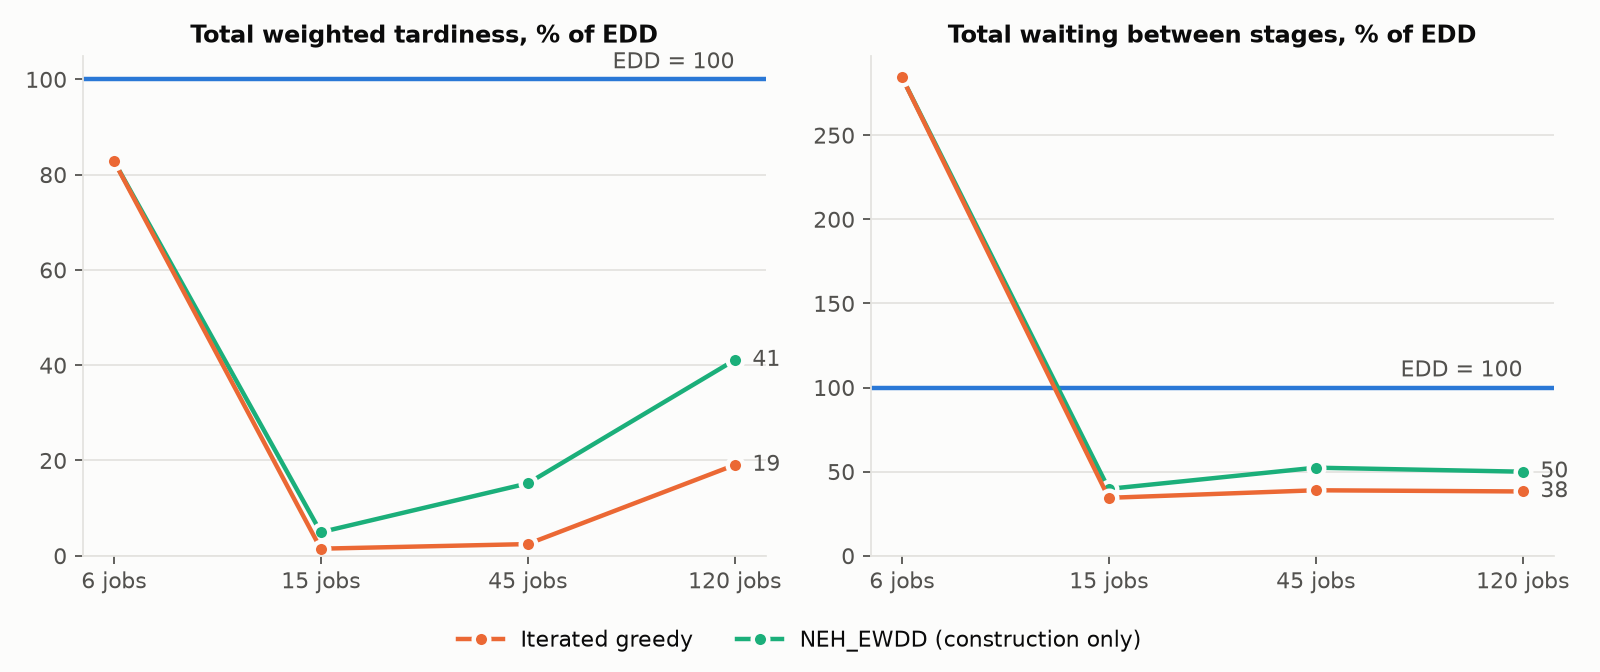
\includegraphics[width=\textwidth]{comparison/comparison.png}
\caption{Total weighted tardiness (left) and total waiting (right) of iterated greedy and of NEH\_EWDD alone, each as a percentage of the EDD value on the same instance (EDD is the line at 100). The horizontal axis gives the instance size; the labels at the right edge are the 120-job values. The two methods coincide on the 6-job instance.}
\label{fig:comparison}
\end{figure}

\sumpara The solver proves the searched values optimal where it can finish, and the seed matters only at 120 jobs. \sumparaend
\fin HiGHS proved the optimal total weighted tardiness to be 233 on the 6-job instance in 0.36~seconds and 21 on the 15-job instance in 85.8~seconds, and iterated greedy reached both values. \fine
\fin On the 15-job instance, the solver's optimal order had 323~minutes of waiting and iterated greedy's had 252, because only iterated greedy breaks ties in $Z$ by waiting. \fine
\fin With seeds 1 to 5, iterated greedy returned exactly the default seed's tardiness on the 6-, 15-, and 45-job instances, and values from 4,159 to 4,306 on the 120-job instance, all below the default seed's 4,383. \fine
\fin Its computation time grew from 0.21~seconds at 6~jobs to 37.2~seconds at 120~jobs, while EDD took under a millisecond on every instance. \fine

\subsection{Paired scenarios at a coefficient of variation of 0.2}\label{sec:stress-results}

\sumpara At a coefficient of variation of 0.2, the searched sequence stays far ahead of the EDD sequence on both measures in every scenario. \sumparaend
\fin \Cref{tab:stress} summarizes the two fixed sequences for the 45-job instance over the 30~saved scenarios at $\nu = 0.2$. \fine
\fin The iterated greedy sequence had the lower weighted tardiness in all 30~scenarios, with a mean of 420.6 weighted minutes against 3,541.1, a reduction of 3,120.5 weighted minutes (standard error 150.1 over the paired scenarios) or 88.1~percent, and a 90th percentile of 592.2 against 4,616.6. \fine
\fin In every scenario the reduction was at least 1,948.6 weighted minutes, and its 10th percentile was 2,235.1. \fine
\fin Its mean waiting was 1,276.9~minutes against 2,454.5, a reduction of 48.0~percent. \fine
\fin Neither sequence violated a hard constraint in any scenario, because right-shift execution preserves release dates, stage order, and one job per stage for any processing times, and due dates are soft targets. \fine
\fin \Cref{fig:stress} shows that the ranges do not overlap: the weighted tardiness of the iterated greedy sequence ranged from 103.3 to 1,120.0, and that of EDD from 2,276.2 to 6,013.8. \fine

\begin{table}[ht]
\centering
\caption{Stress test on the 45-job instance: 30~scenarios at a coefficient of variation of 0.2, seed 20261103. ``Planned'' is the value of the sequence on the exact data; the mean and the 90th percentile are over the scenarios. Tardiness is in weighted minutes and waiting in minutes.}
\label{tab:stress}
\small
\begin{tabular}{lrrrrrrr}
\toprule
 & \multicolumn{3}{c}{Total weighted tardiness} & \multicolumn{3}{c}{Total waiting} & Scenarios breaking \\
\cmidrule(lr){2-4}\cmidrule(lr){5-7}
Sequence & Planned & Mean & 90th pct. & Planned & Mean & 90th pct. & a hard constraint \\
\midrule
Earliest due date & 2,371.0 & 3,541.1 & 4,616.6 & 2,040.0 & 2,454.5 & 2,768.6 & 0 \\
Iterated greedy & 58.0 & 420.6 & 592.2 & 794.0 & 1,276.9 & 1,454.9 & 0 \\
\bottomrule
\end{tabular}
\end{table}

\begin{figure}[ht]
\centering
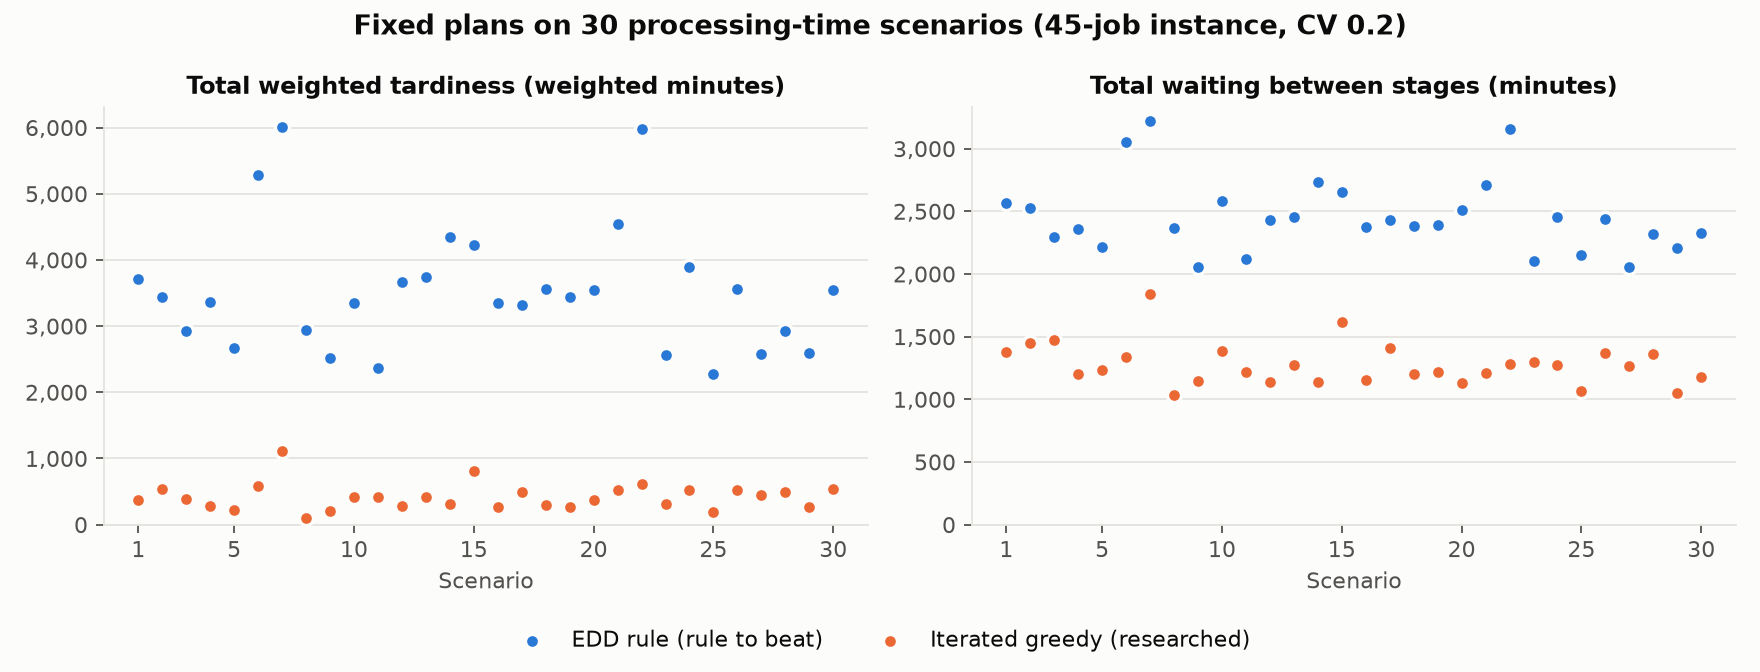
\includegraphics[width=\textwidth]{stress/stress_per_scenario.png}
\caption{Total weighted tardiness (left) and total waiting (right) of the two fixed sequences in each of the 30~scenarios of \cref{tab:stress}. Each dot is one sequence in one scenario, and both sequences face the same realized processing times in a scenario.}
\label{fig:stress}
\end{figure}

\subsection{Sensitivity to processing-time variability}\label{sec:sweep}

\sumpara Higher variability raises the tardiness of both sequences, cuts the relative advantage, and thins the worst periods' gain, while the mean gain holds. \sumparaend
\fin \Cref{tab:sweep} and \cref{fig:sweep} repeat the execution at five coefficients of variation, each with 30~new scenarios. \fine
\fin The mean weighted tardiness of the iterated greedy sequence rose from 148.1 at $\nu = 0.1$ to 8,901.6 at $\nu = 0.8$, and that of EDD from 2,720.1 to 12,230.5. \fine
\fin The relative reduction in mean weighted tardiness fell from 94.6~percent at $\nu = 0.1$ to 27.2~percent at $\nu = 0.8$. \fine
\fin The mean absolute reduction stayed between 2,572.0 and 3,683.7 weighted minutes at every level: it rose from $\nu = 0.1$ (standard error 65.9) to $\nu = 0.5$ (standard error 223.8), and its fall of 354.8 to 3,329.0 at $\nu = 0.8$ (standard error 342.7) is within the combined standard error of 409.3 of the two estimates. \fine
\fin The gain in a single period became less dependable at $\nu = 0.8$: the 10th percentile of the per-scenario reduction, between 1,781.1 and 2,473.2 weighted minutes at the lower levels, fell to 851.5, and the EDD sequence won 1 of the 30~scenarios, by 870.4 weighted minutes, its only win in the 180 paired scenarios of the six sets. \fine

\begin{table}[ht]
\centering
\caption{Sweep over variability on the 45-job instance. Each row uses 30~new scenarios, from seeds 6522 to 6526 in order. Tardiness is in weighted minutes. The reduction is the per-scenario difference between the two sequences' weighted tardiness: its mean, with the standard error in parentheses, and its 10th percentile; the percentage compares the two sequences' means.}
\label{tab:sweep}
\small
\setlength{\tabcolsep}{4.5pt}
\begin{tabular}{rrrrrrrr}
\toprule
 & \multicolumn{2}{c}{Earliest due date} & \multicolumn{2}{c}{Iterated greedy} & \multicolumn{3}{c}{Reduction} \\
\cmidrule(lr){2-3}\cmidrule(lr){4-5}\cmidrule(lr){6-8}
$\nu$ & Mean & 90th pct. & Mean & 90th pct. & Mean (s.e.) & 10th pct. & Percent \\
\midrule
0.1 & 2,720.1 & 3,171.6 & 148.1 & 228.4 & 2,572.0 (65.9) & 2,048.3 & 94.6 \\
0.2 & 3,273.5 & 4,425.0 & 407.2 & 643.9 & 2,866.4 (121.3) & 2,055.3 & 87.6 \\
0.3 & 4,139.8 & 6,213.4 & 952.5 & 1,676.0 & 3,187.3 (203.8) & 1,781.1 & 77.0 \\
0.5 & 6,680.4 & 9,498.8 & 2,996.7 & 5,434.2 & 3,683.7 (223.8) & 2,473.2 & 55.1 \\
0.8 & 12,230.5 & 17,420.0 & 8,901.6 & 14,219.8 & 3,329.0 (342.7) & 851.5 & 27.2 \\
\bottomrule
\end{tabular}
\end{table}

\begin{figure}[ht]
\centering
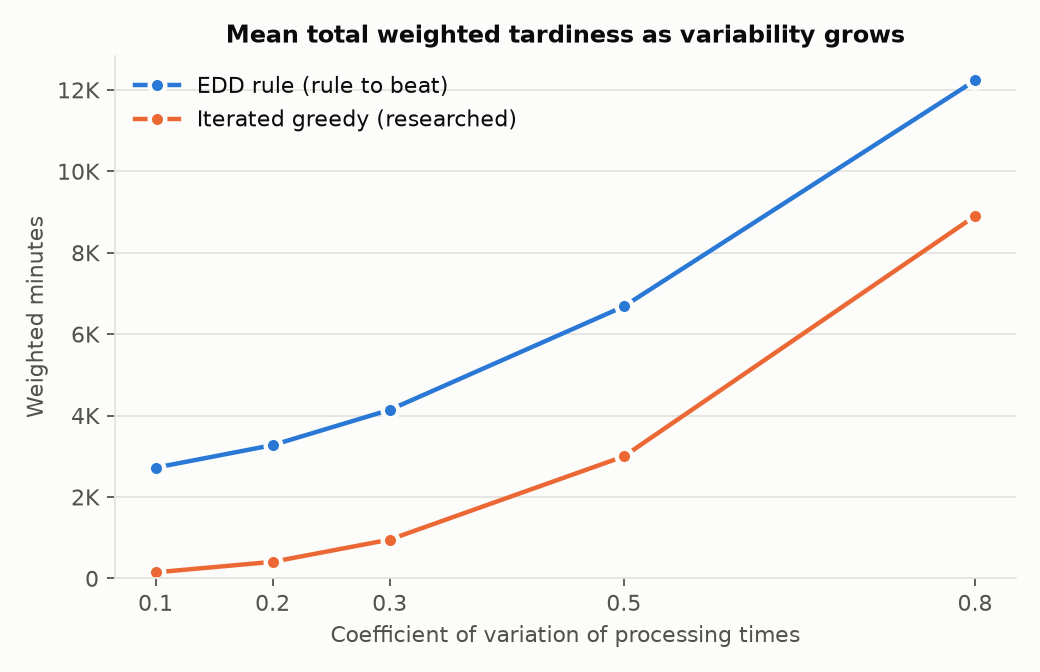
\includegraphics[width=0.62\textwidth]{stress/stress_cv_sweep.png}
\caption{Mean total weighted tardiness of the two fixed sequences for the 45-job instance at five coefficients of variation of the processing times, 30~scenarios each (\cref{tab:sweep}). The vertical gap between the lines is the absolute reduction, between 2,572.0 and 3,683.7 weighted minutes at every level.}
\label{fig:sweep}
\end{figure}

\section{Discussion}\label{sec:discussion}

\subsection{Sources of the deterministic improvement}\label{sec:gain}

\sumpara On the 6-job instance, the gain comes from moving a low-weight job behind two high-weight jobs. \sumparaend
\fin \Cref{fig:gantt} draws both schedules of the 6-job instance. \fine
\fin EDD places job J005, due at 67 with weight 1, ahead of jobs J003 and J004, which carry weight 4. \fine
\fin Iterated greedy moves J005 to the end, so J003 finishes at 97 and J004 at 119, against 108 and 139 under EDD, while J005 finishes at 136, against 82. \fine
\fin The weighted tardiness of J003 and J004 falls by 124 weighted minutes and that of J005 rises by 54, and with a smaller rise for J006 the total falls from 281 to 233. \fine
\fin The same reordering raises waiting on this instance from 13 to 37~job-minutes, because the two jobs now at the end, J006 and J005, wait 18 and 19~minutes at stages S2 to S4 behind the long operations of the weight-4 jobs. \fine

\begin{figure}[ht]
\centering
{\footnotesize\color{muted}Earliest due date: J001, J002, J005, J003, J006, J004 (total weighted tardiness 281)}\\[2pt]
\gantt{\eddschedule}\\[6pt]
{\footnotesize\color{muted}Iterated greedy: J001, J002, J003, J004, J006, J005 (total weighted tardiness 233, the optimum)}\\[2pt]
\gantt{\igschedule}\\[4pt]
{\footnotesize\color{muted}Shading gives the job's weight:
\textcolor{w1}{\rule{0.7em}{0.7em}}~1\quad
\textcolor{w2}{\rule{0.7em}{0.7em}}~2\quad
\textcolor{w4}{\rule{0.7em}{0.7em}}~4}
\caption{Both schedules of the 6-job instance on stages S1 to S4, with time in minutes on the horizontal axis. Each bar is one operation, labeled with its job number and shaded by the job's weight. Iterated greedy moves the weight-1 job J005 behind the weight-4 jobs J003 and J004.}
\label{fig:gantt}
\end{figure}

\sumpara On the development instances, weighting turns most late jobs into on-time jobs, and the search removes most of the tardiness that the weighted start leaves. \sumparaend
\fin The share of jobs finishing on time rises from 0.333, 0.244, and 0.233 under EDD to 0.867, 0.911, and 0.642 under iterated greedy on the instances with 15, 45, and 120~jobs. \fine
\fin NEH\_EWDD alone already lowers weighted tardiness relative to EDD by 95.1, 84.8, and 58.9~percent on these instances (\cref{tab:comparison}), and the iterations of \cref{alg:ig} lower its value by a further 70.0, 83.9, and 53.6~percent, or 49, 302, and 5,069 weighted minutes. \fine
\fin On the 120-job instance the search has not converged after 5000~iterations, since five other seeds find sequences 1.8 to 5.1~percent better than the default seed's 4,383, at a computation time that already reaches 37.2~seconds. \fine
\fin On the 15-job instance, the solver returned one optimal order, with tardiness 21 and, under earliest-start execution, 323~job-minutes of waiting, and the order found by iterated greedy has the same tardiness and 252~job-minutes. \fine
\fin This difference of 71~job-minutes of interstage waiting is relative to that particular solver solution: the program minimizes $Z$ alone, so another optimal order could have more or less waiting. \fine

\subsection{On-time jobs under processing-time variability}\label{sec:loss}

\sumpara Under variability the searched sequence loses on-time jobs, while the EDD sequence mainly lengthens lateness it already has. \sumparaend
\fin At $\nu = 0.2$, the iterated greedy sequence has 4 late jobs as planned and 11.5 on average across the 30~scenarios, while the EDD sequence has 34 and 36.1. \fine
\fin The mean weighted tardiness of EDD rises by 1,170.1 weighted minutes over its planned value while its count of late jobs rises by only 2.1, so most of its increase comes from jobs that were already late finishing later still. \fine
\fin The mean of the iterated greedy sequence rises by 362.6, a factor of 7.25 over its planned 58, against a factor of 1.49 for EDD, because its losses come from jobs that were on time in the plan. \fine
\fin Because the mean of EDD rises by more in absolute terms, the mean reduction at this level exceeds the planned gap of 2,313 weighted minutes; these late-job statistics are measured at $\nu = 0.2$ only, so they do not speak to the higher levels. \fine

\sumpara Each on-time job of the searched sequence is less likely to turn late than one of EDD, and the sequence loses more because it has more of them. \sumparaend
\fin The on-time jobs of the iterated greedy sequence have a median planned slack of 31~minutes before their due dates, against 28 for EDD. \fine
\fin To include the delays passed on by the jobs ahead, we measure each on-time job's completion at the last stage across the 30~saved scenarios at $\nu = 0.2$: its mean moves later than planned by a median of 9.3~minutes for iterated greedy and 3.5 for EDD, and its standard deviation has a median of 8.3~minutes and 9.9, respectively. \fine
\fin Slack falls below one such standard deviation for 6 of the 41 on-time jobs of iterated greedy and for 4 of the 11 of EDD. \fine
\fin An on-time job of the iterated greedy sequence finishes late in 18.5~percent of the scenarios on average, against 27.9~percent for EDD, but with 41 such jobs against 11, an average of 7.6 turn late per scenario, against 3.1. \fine
\fin This mechanism is consistent with the observation of \citet{aytug2005executing} that optimized schedules lose their advantage as variability grows, and the sweep shows that, for weighted tardiness on this instance, the relative reduction falls at every level tested while the mean absolute reduction does not. \fine
\fin It parallels, for this objective and without a stochastic comparator, the finding of \citet{framinan2015stochastic} and \citet{juan2014simheuristic} for the expected makespan that sequences computed on exact or mean processing times remain effective at low to moderate variability. \fine

\subsection{Implications, scope, and extensions}\label{sec:implications}

\sumpara A planner should adopt the searched sequence and monitor the line's variability. \sumparaend
\fin For a planning period like the 45-job instance with processing times varying at a coefficient of variation of 0.2, the iterated greedy sequence lowers mean total weighted tardiness relative to the frozen EDD list by 3,120.5 weighted minutes (standard error 150.1) in the main scenarios and by 2,866.4 (standard error 121.3) in an independent second set, leaves 11.5~jobs late per period on average against 36.1, and lowers mean waiting between stages by 48.0~percent. \fine
\fin In exchange, the planner gives up a sequence that can be traced by hand and accepts a result that depends on a seed and takes seconds to compute, 3.22 at 45~jobs and 37.2 at 120. \fine
\fin At $\nu = 0.8$ the mean gain remains 3,329.0 weighted minutes, but the 10th percentile of the per-period gain falls to 7.0~percent of the EDD mean and EDD is better in 1 of 30~scenarios, so a planner who weighs the worst periods most should repeat the comparison at the line's measured variability. \fine

\sumpara The design bounds the claim in five ways. \sumparaend
\fin All four instances come from one generator, with processing times of 2 to 20~minutes and median due-date windows of 154 to 158~minutes, and the stress test covers only the 45-job instance, so lines with tighter due dates or more uneven stages may show different margins. \fine
\fin The scenarios draw each of the 360 processing times of the 45-job instance independently, so they do not represent a common cause, such as a slow shift or a degraded machine, that lengthens many operations at once, and they replicate processing-time noise for one pair of sequences on one instance, which does not replicate the comparison across instances. \fine
\fin Both sequences are predictive and are never revised, which isolates the value of the sequence itself and leaves out rescheduling and reactive dispatching; in the studies reviewed by \citet{aytug2005executing}, dispatching matched or outperformed predictive schedules once variability was high. \fine
\fin Optimality is proven only up to 15~jobs, and on the 120-job instance other seeds find better sequences, so the gains reported for the largest instance understate what the search can achieve. \fine
\fin NEH\_EWDD, which involves no search, was not executed in the scenarios and no stochastic method was run, so the stress test does not separate the contribution of the search from that of the weighted start or compare the sequence with a method that samples scenarios. \fine

\sumpara Each limit points to one extension with a direct test. \sumparaend
\fin A search that scores each candidate sequence by its mean tardiness over sampled scenarios, in the manner of the simheuristic of \citet{juan2014simheuristic}, would target the variability directly, and the sweep of \cref{sec:sweep} provides the test. \fine
\fin Scenarios with correlated factors, in which one draw lengthens a whole stage or a whole shift, would test whether the absolute gain survives a common cause. \fine
\fin Re-sequencing at each release with the processing times already realized would measure how much of the loss under variability a predictive-reactive policy recovers. \fine

\section{Conclusions}\label{sec:conclusions}

\sumpara Three results are now established for this line. \sumparaend
\fin On exact data, iterated greedy reduced total weighted tardiness relative to EDD by 81.0 to 98.5~percent on the development instances and attained the proven optimum on both instances for which we certified one. \fine
\fin Executed unchanged while processing times varied with a coefficient of variation of 0.2, the searched sequence had the lower weighted tardiness in all 30~scenarios and an 88.1~percent lower mean. \fine
\fin As the coefficient of variation rose to 0.8, the relative reduction fell to 27.2~percent and the 10th percentile of the per-period reduction to 851.5 weighted minutes, while the mean absolute reduction stayed between 2,572.0 and 3,683.7 weighted minutes. \fine

\sumpara The contribution is paired evidence on how variability changes the value of a fixed iterated greedy sequence. \sumparaend
\fin For a planner who must fix one sequence before processing begins, we found on this instance that the mean gain of an iterated greedy sequence over a frozen EDD list held at every level of processing-time variability we tested, and that variability, the one factor we varied, determined how dependably that gain was realized in a single period. \fine

\paragraph{Data availability.}
\fin The code, the data, every schedule, and every result reported here are publicly available at \url{https://github.com/mutingma123/OM522Project}, where one command regenerates every table and figure. \fine


\phantomsection\addcontentsline{toc}{section}{References}
\bibliographystyle{unsrtnat}
\bibliography{Option6_Report}

\appendix
\section{Notation}\label{sec:notation}

\sumpara The three tables list every symbol once, with its meaning and units. \sumparaend
\fin \Cref{tab:notation-data,tab:notation-schedule,tab:notation-method} list every symbol in the report with its meaning, its units, and where it is defined. \fine
\fin No symbol carries two meanings. \fine

\begin{table}[!htbp]
\centering
\caption{Indices and data.}
\label{tab:notation-data}
\small
\begin{tabularx}{\textwidth}{lLll}
\toprule
Symbol & Meaning & Units & Defined in \\
\midrule
$n$ & Number of jobs & jobs & \cref{sec:timing} \\
$m$ & Number of stages & stages & \cref{sec:timing} \\
$j$ & Job index, $j = 1, \ldots, n$ & & \cref{sec:timing} \\
$h$ & Job index in sums and maxima that already involve $j$ & & \cref{sec:mip} \\
$k$ & Stage index in line order, $k = 1, \ldots, m$ & & \cref{sec:timing} \\
$i$ & Position index within a sequence $\pi$ & & \cref{sec:timing} \\
$q$ & Position index in the mixed-integer program & & \cref{sec:mip} \\
$r_j$ & Release time of job $j$ & minutes & \cref{sec:timing} \\
$d_j$ & Due date of job $j$ & minutes & \cref{sec:timing} \\
$w_j$ & Weight (priority score) of job $j$ & integer score & \cref{sec:timing} \\
$p_{jk}$ & Processing time of job $j$ at stage $k$ & minutes & \cref{sec:timing} \\
\bottomrule
\end{tabularx}
\end{table}

\begin{table}[!htbp]
\centering
\caption{Schedules, measures, and variables of the mixed-integer program.}
\label{tab:notation-schedule}
\small
\begin{tabularx}{\textwidth}{lLll}
\toprule
Symbol & Meaning & Units & Defined in \\
\midrule
$\pi$, $\pi(i)$ & A sequence of all jobs, and the job in its position $i$ & & \cref{sec:timing} \\
$S_{jk}$, $C_{jk}$ & Start and completion of job $j$ at stage $k$ & minutes & \eqref{eq:recursion} \\
$T_j$ & Tardiness of job $j$, $\max\{0, C_{jm} - d_j\}$ & minutes & \cref{sec:timing} \\
$Z(\pi)$ & Total weighted tardiness of $\pi$ (primary measure) & weighted minutes & \eqref{eq:measures} \\
$W(\pi)$ & Total waiting between stages of $\pi$ (secondary measure) & minutes & \eqref{eq:measures} \\
$F(\pi)$ & The pair $(Z(\pi), W(\pi))$, compared lexicographically & & \cref{sec:methods} \\
$x_{jq}$ & 1 if job $j$ takes position $q$, 0 otherwise & binary & \cref{sec:mip} \\
$B_{qk}$, $E_{qk}$ & Start and end of the job in position $q$ at stage $k$ & minutes & \cref{sec:mip} \\
$U_j$ & Upper bound on the tardiness of job $j$ in \eqref{eq:mip-tardy} & minutes & \cref{sec:mip} \\
\bottomrule
\end{tabularx}
\end{table}

\begin{table}[!htbp]
\centering
\caption{Method and experiment settings.}
\label{tab:notation-method}
\small
\begin{tabularx}{\textwidth}{lLll}
\toprule
Symbol & Meaning & Value or units & Defined in \\
\midrule
$\pi^{\mathrm{EDD}}$ & Sequence of the earliest due date rule & & \cref{alg:ig} \\
$\pi^{*}$, $\pi'$, $\pi''$ & Best sequence found, a rebuilt sequence, and a local search candidate & & \cref{alg:ig} \\
$\delta$ & Number of jobs removed in each iteration & 4 & \cref{sec:methods} \\
$\lambda$ & Temperature factor & 0.5 & \cref{sec:methods} \\
$\Theta$ & Temperature, $\lambda \sum_{j,k} p_{jk} / (10\, n\, m)$, compared with increases in $Z$ & minutes & \cref{sec:methods} \\
$\Delta$ & Increase in $Z$ of a candidate over the current sequence & weighted minutes & \cref{sec:methods} \\
$L$, $\ell$ & Iteration limit and iteration counter & $L = 5000$ & \cref{alg:ig} \\
$u$ & Uniform random draw on $[0, 1]$ in the acceptance test & & \cref{alg:ig} \\
$\omega$ & Scenario index & 30 per test & \cref{sec:stress-design} \\
$\varepsilon_{jk\omega}$ & Lognormal factor on $p_{jk}$ in scenario $\omega$, mean 1 & & \cref{sec:stress-design} \\
$\nu$ & Coefficient of variation of each factor & 0.1 to 0.8 & \cref{sec:stress-design} \\
$\sigma$ & Standard deviation of $\ln \varepsilon_{jk\omega}$, $\sigma^2 = \ln(1 + \nu^2)$ & & \cref{sec:stress-design} \\
\bottomrule
\end{tabularx}
\end{table}

\end{document}
